\documentclass{sciposter}
\usepackage{lipsum}
\usepackage{epsfig}
\usepackage{amsmath}
\usepackage{amssymb}
\usepackage{multicol}
\usepackage{graphicx,url}
%\usepackage[portuges, brazil]{babel}   
\usepackage[utf8]{inputenc}
%\usepackage{fancybullets}
\newtheorem{Def}{Definition}


\title{Performance Analysis of Undefined Behavior Optimizations}
\author{*Lucian I. Popescu, **Nuno P. Lopes}

\institute 
{
*Faculty of Automatic Control and Computer Science,\\
Politehnica University of Bucharest \\
** Instituto Superior Técnico, \\
Universidade de Lisboa
}

\email{*lucian.popescu187@gmail.com, **nuno.lopes@tecnico.ulisboa.pt}

% TODO: change them with higher resolution logos
\rightlogo[1]{logo-upb}
\leftlogo[1]{logo-ist}


\begin{document}

\conference{{\bf EuroLLVM 23}, 11th May 2023, Glasgow, GB}

%\LEFTSIDEfootlogo  
% Uncomment to put footer logo on left side, and 
% conference name on right side of footer

% Some examples of caption control (remove % to check result)

%\renewcommand{\algorithmname}{Algoritme} % for Dutch

%\renewcommand{\mastercapstartstyle}[1]{\textit{\textbf{#1}}}
%\renewcommand{\algcapstartstyle}[1]{\textsc{\textbf{#1}}}
%\renewcommand{\algcapbodystyle}{\bfseries}
%\renewcommand{\thealgorithm}{\Roman{algorithm}}

\maketitle

\begin{multicols}{3}

\section{Introduction}
Clang and LLVM use undefined behavior (UB) to issue code optimizations.
Currently, there is no study that evaluates the performance impact of this class
of optimizations. We fill this gap by presenting some early results in this
area. Phoronix Test Suite was used to evaluate the performance of a diverse set
of applications, including webservers, compression algorithms, graphical
environments, etc. By compiling each application with flags that trigger
specific UBs, we gathered various metrics (requests per second, MB/s, FPS,
etc) for further analysis. Early results show that in nearly 90\% of the cases
the performance impact is insignificant (between -2\% and 2\%).
\begin{figure}[h!]
\centering
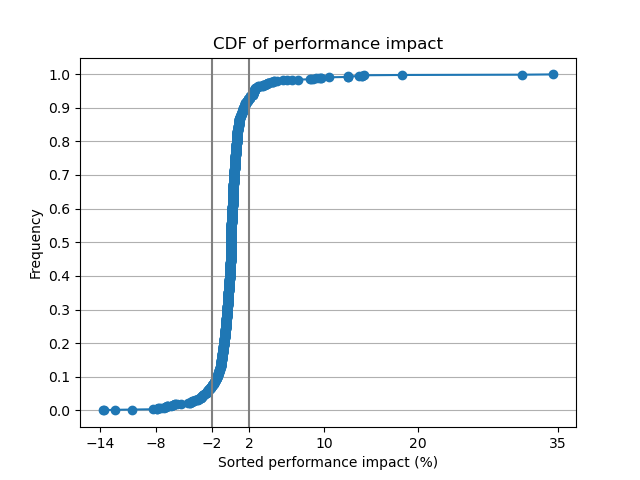
\includegraphics[scale=1.2]{perf-cdf}
\caption{CDF of performance impact for all UB flags}
\end{figure}

\section{Experiment Setup}
The performance tests were run on a machine with the following specs:
\begin{itemize}
\item Processor: 2 x Intel Xeon E5-2680 v2 @ 3.60GHz (20 Cores / 40 Threads)
\item Motherboard: HP 158A (J61 v03.69 BIOS)
\item Chipset: Intel Xeon E7 v2/Xeon
\item Memory: 8 x 8 GB DDR3-1600MT/s HMT41GR7AFR4A-PB
\item Disk: 2000GB TOSHIBA DT01ACA2
\item Graphics: NVIDIA NVE4 4GB
\item OS: Debian 11
\item Kernel: 5.10.0-21-amd64 (x86\_64)
\item Display Server: X Server 1.20.11
\item Display Driver: nouveau
\item Compiler: Clang 15.0.7 + LLVM 15.0.7
\item File-System: ext4
\item Screen Resolution: 1920x1080
\end{itemize}
\bigbreak
\bigbreak
The experiments were conducted using the following steps:
\begin{itemize}
\item Compile the benchmark with no UB flags enabled (baseline)
\item Compile the benchmark using one UB flag at a time
\item Run baseline using Phoronix and fetch the results
\item Run the benchmarks with UB flags using Phoronix and fetch the results
\item Compare the UB flags benchmark results with the baseline
\end{itemize}

\section{Undefied Behavior flags}

\subsection{Existing flags}
\textbf{-fwrapv} Treat signed integer overflow as two's complement. Stops the compiler
from optimizing loops and TODO \\
\begin{figure}[h!]
\centering
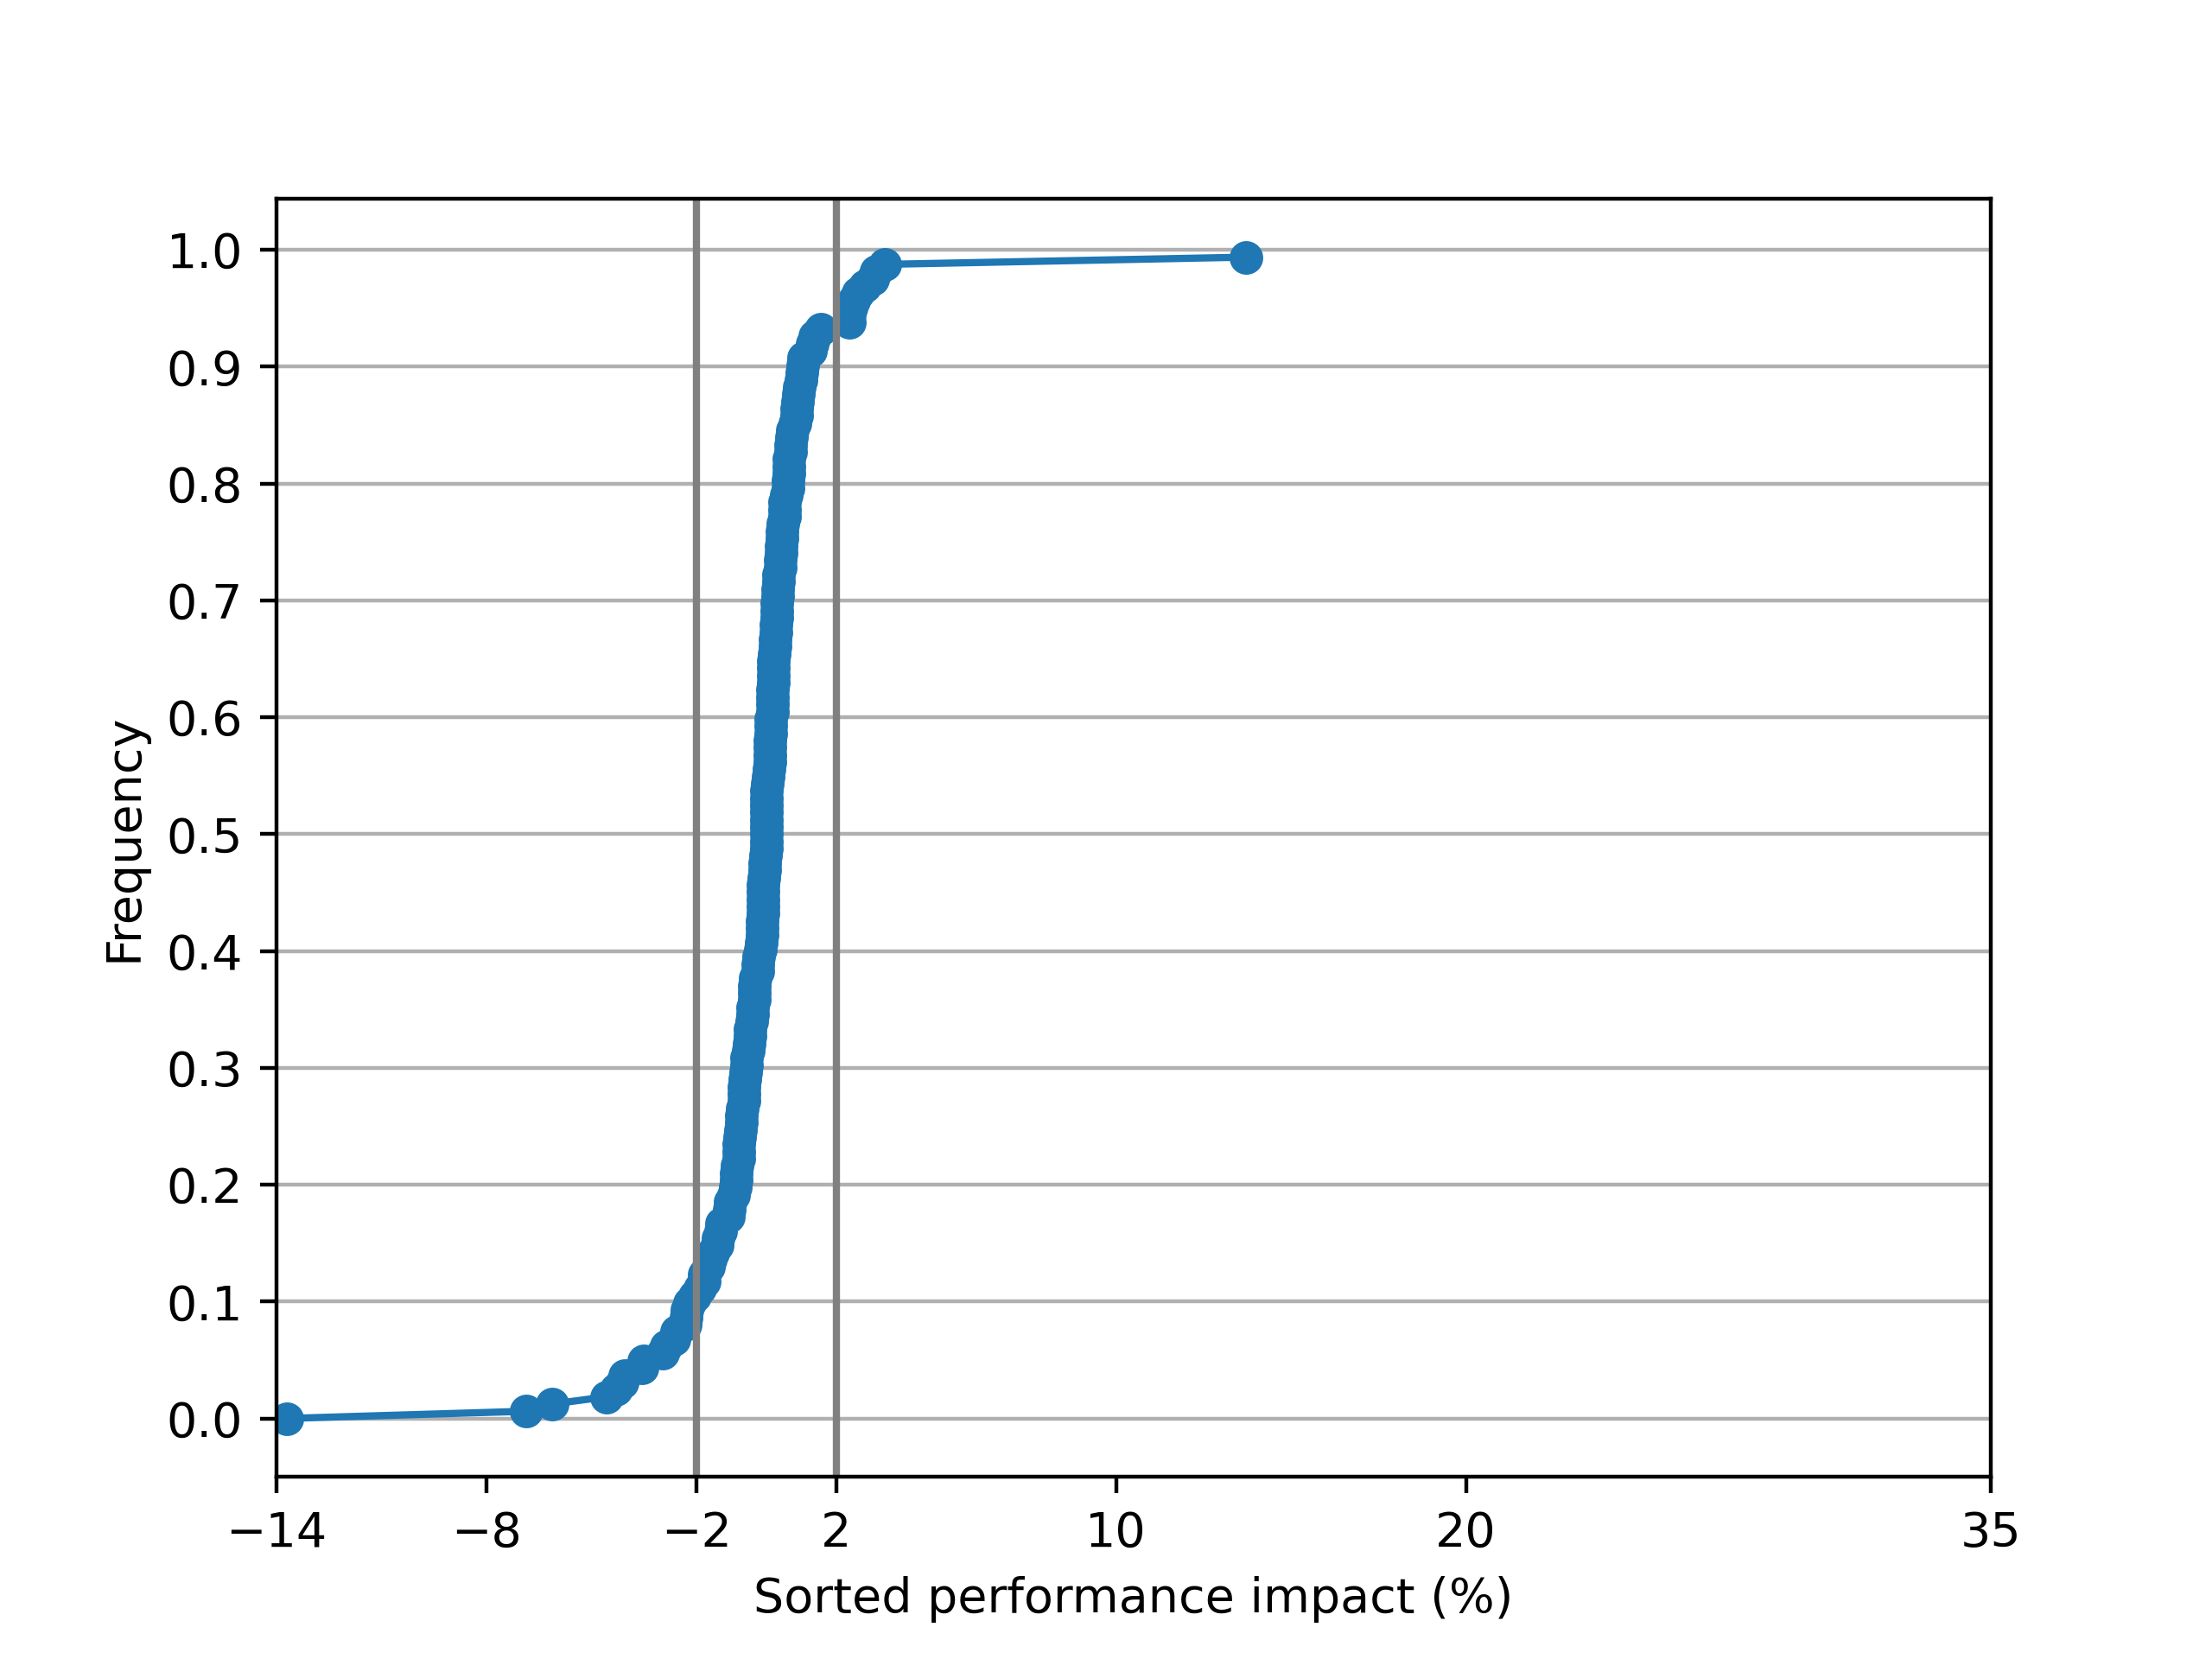
\includegraphics[scale=1.2]{fwrapv}
\caption{CDF of performance impact for fwrapv}
\end{figure}

\textbf{-fno-strict-aliasing} Drop the strictest aliasing rules applicable to
the language being compiled. \\
\begin{figure}[h!]
\centering
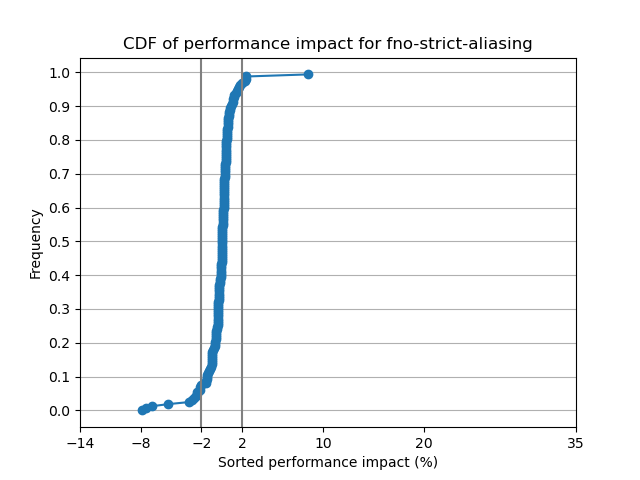
\includegraphics[scale=1.2]{fno-strict-aliasing}
\caption{CDF of performance impact for fno-strict-aliasing}
\end{figure}

\textbf{-fstrict-enums} Enable optimizations based on the strict definition of
an enum's value range. \\
\begin{figure}[h!]
\centering
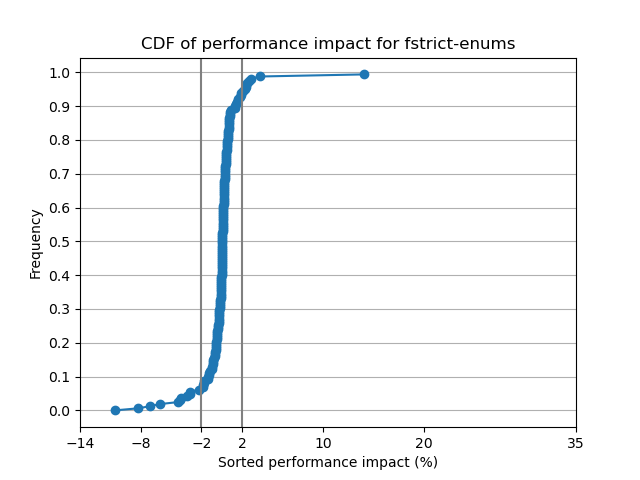
\includegraphics[scale=1.2]{fstrict-enums}
\caption{CDF of performance impact for fstrict-enums}
\end{figure}

\textbf{-fno-delete-null-pointer-checks} Assume that programs can safely
dereference null pointers, and that code or data elements may resides at address
zero. This disables the deletion of "redundant" NULL pointer checks.\\
\begin{figure}[h!]
\centering
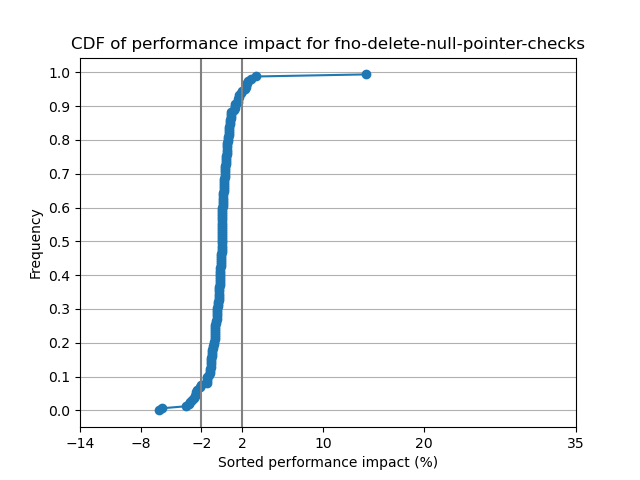
\includegraphics[scale=1.2]{fno-delete-null-pointer-checks}
\caption{CDF of performance impact for fno-delete-null-pointer-checks}
\end{figure}
%\textbf{-fno-finite-loops} \\
%\includegraphics{fno-finite-loops} \\

\subsection{Flags added by us}
\textbf{-fconstrain-shift-value} Shift amount is required to be at most the word
size of LHS. An additional 'and' instruction is inserted.\\
\begin{figure}[h!]
\centering
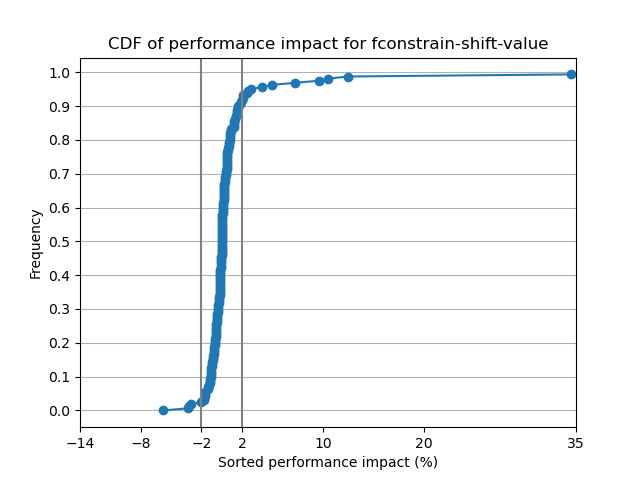
\includegraphics[scale=1.2]{fconstrain-shift-value}
\caption{CDF of performance impact for fconstrain-shift-value}
\end{figure}

\textbf{-fno-constrain-bool-value} Do not constrain bool values in {0,1}.
Instead of using LLVM's range metadata, an additional 'and' instruction is
inserted.\\
\begin{figure}[h!]
\centering
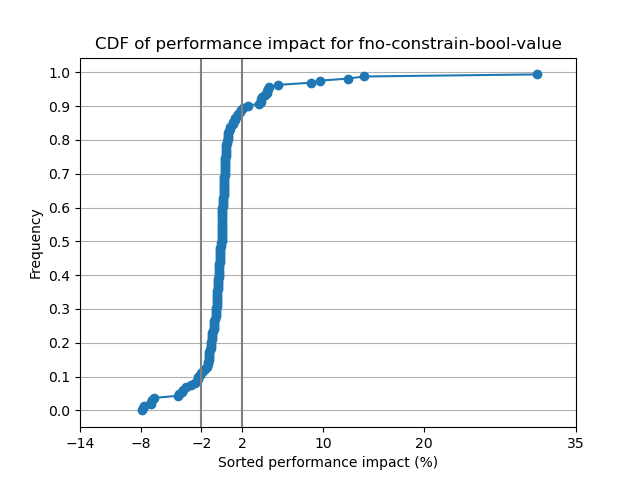
\includegraphics[scale=1.2]{fno-constrain-bool-value}
\caption{CDF of performance impact for fno-constrain-bool-value}
\end{figure}

\textbf{-fno-use-default-alignment} Use alignment of 1 for all memory operations
including load, store, memcpy et al. Global variables and alloca's remain
unaffected.\\
\begin{figure}[h!]
\centering
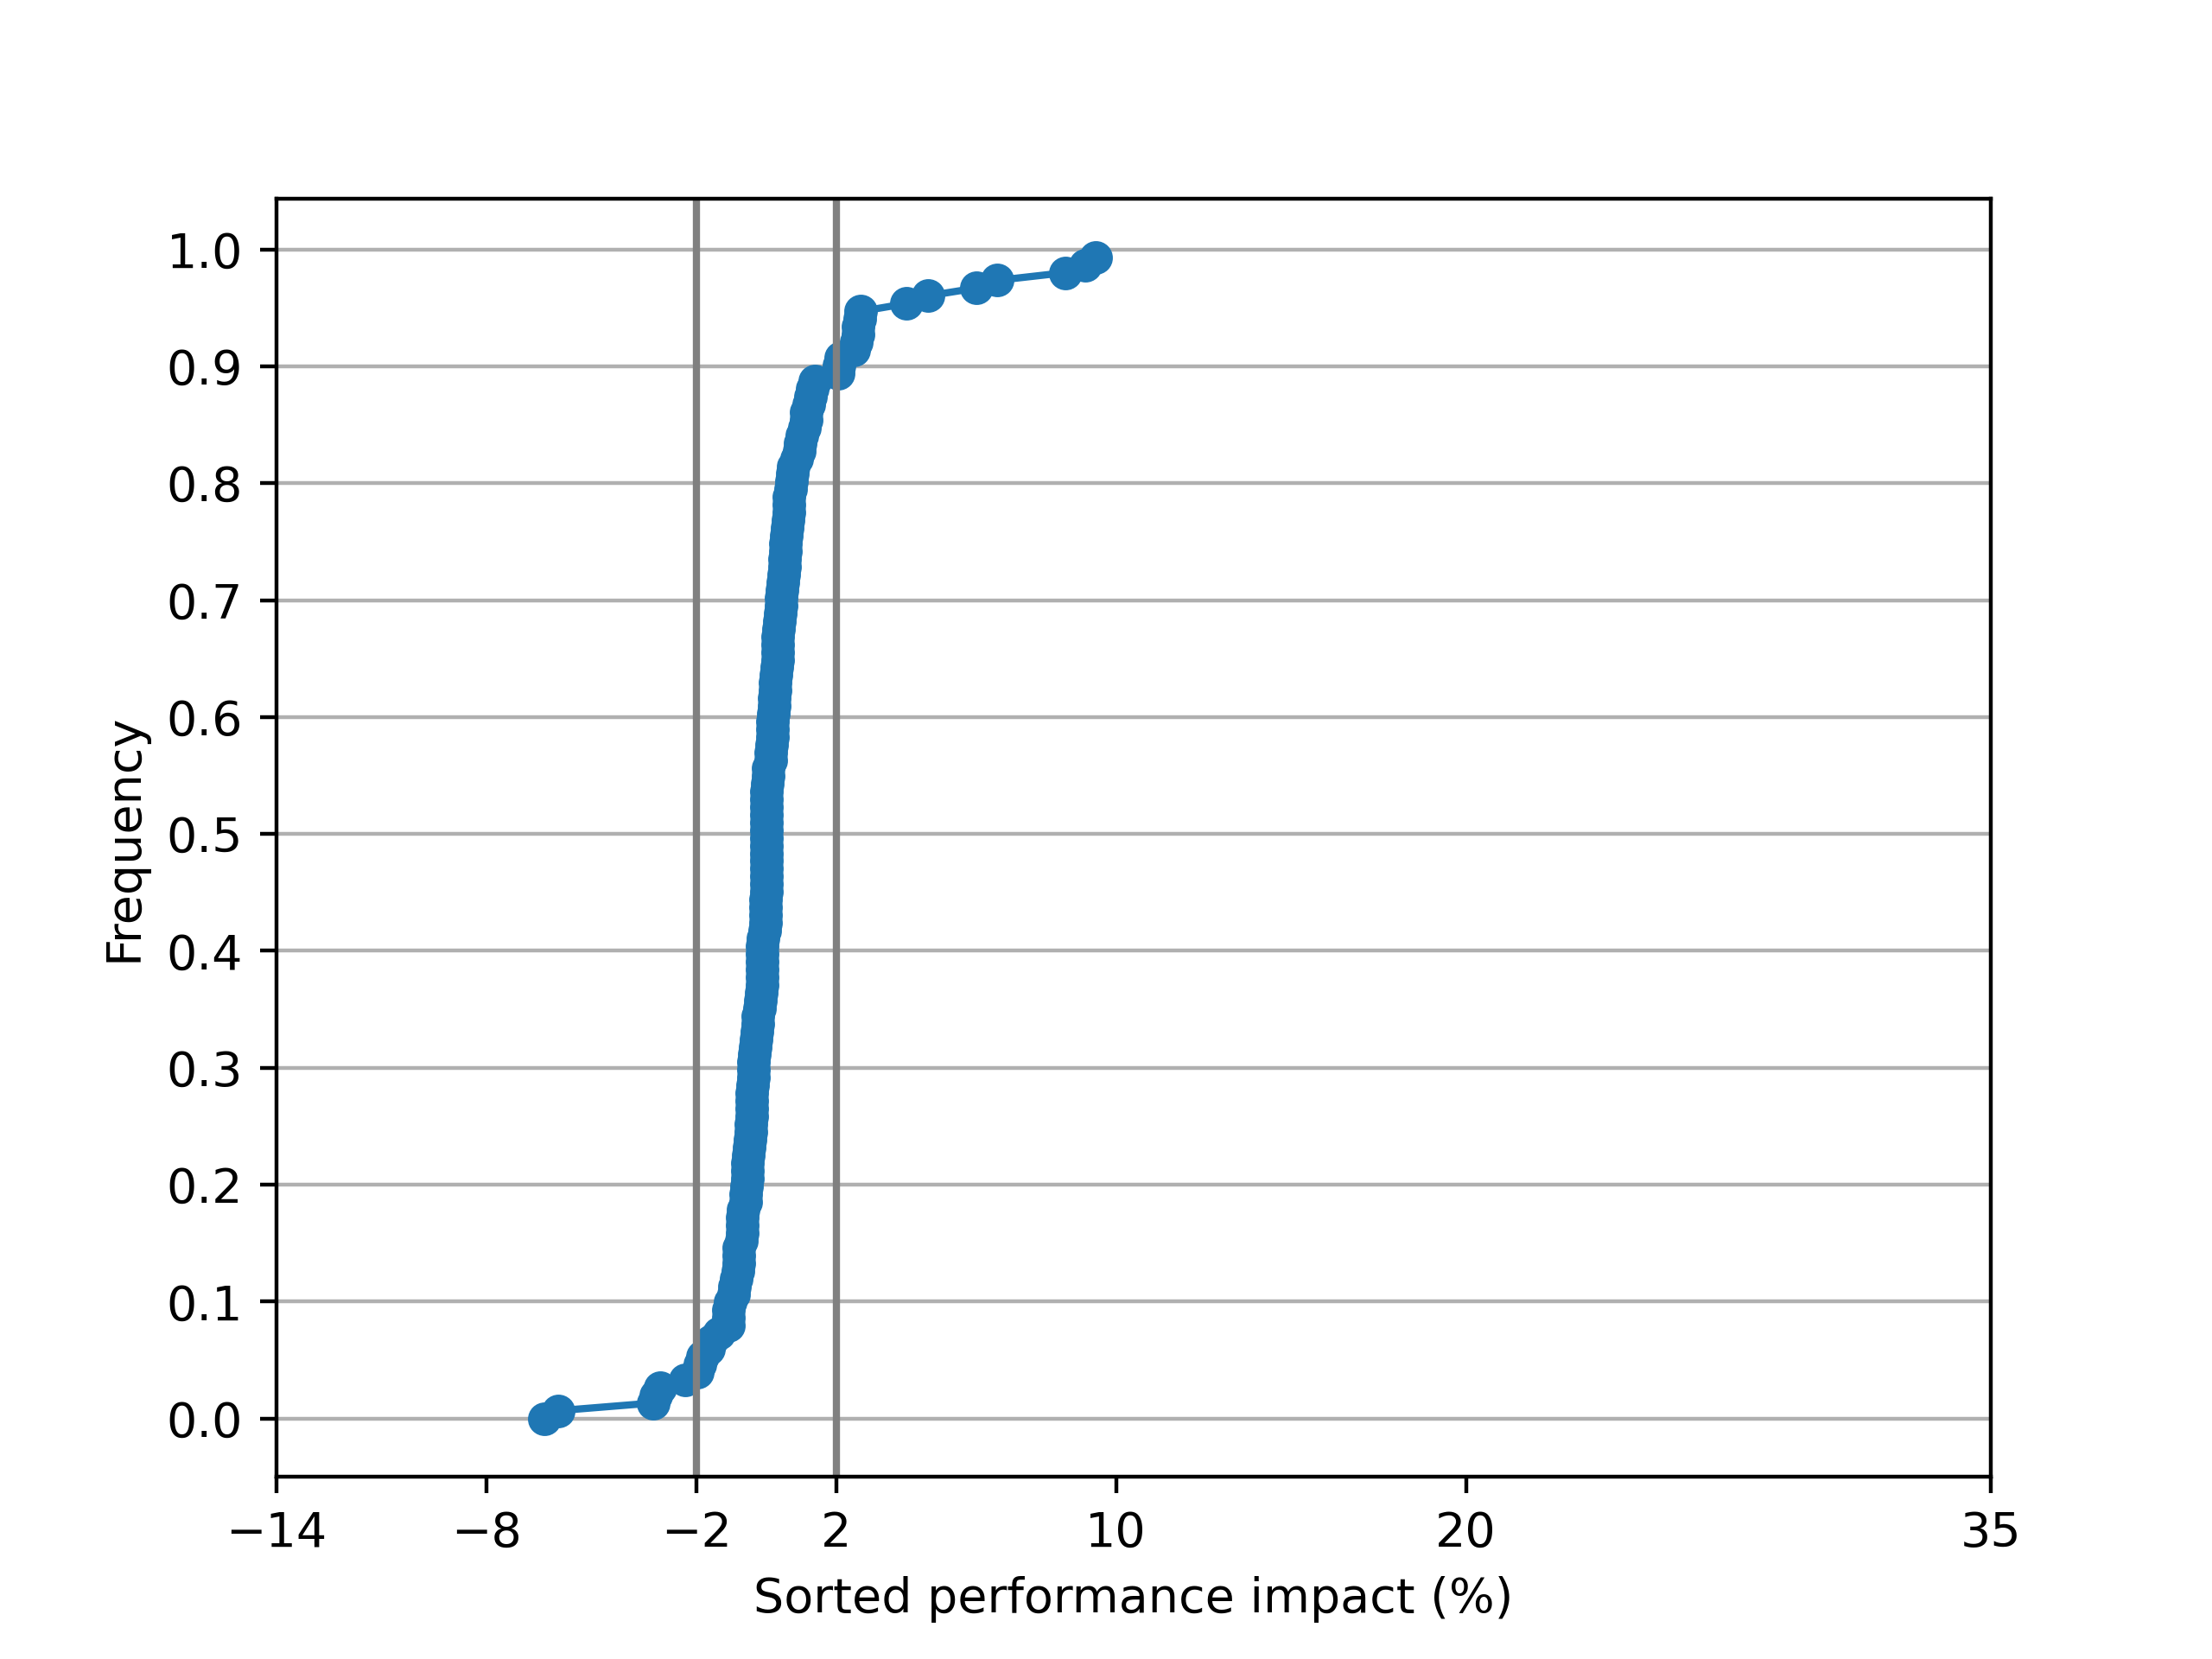
\includegraphics[scale=1.2]{fno-use-default-alignment}
\caption{CDF of performance impact for fno-use-default-alignment}
\end{figure}

\section{Outliers}
\begin{figure}[h!]
\centering
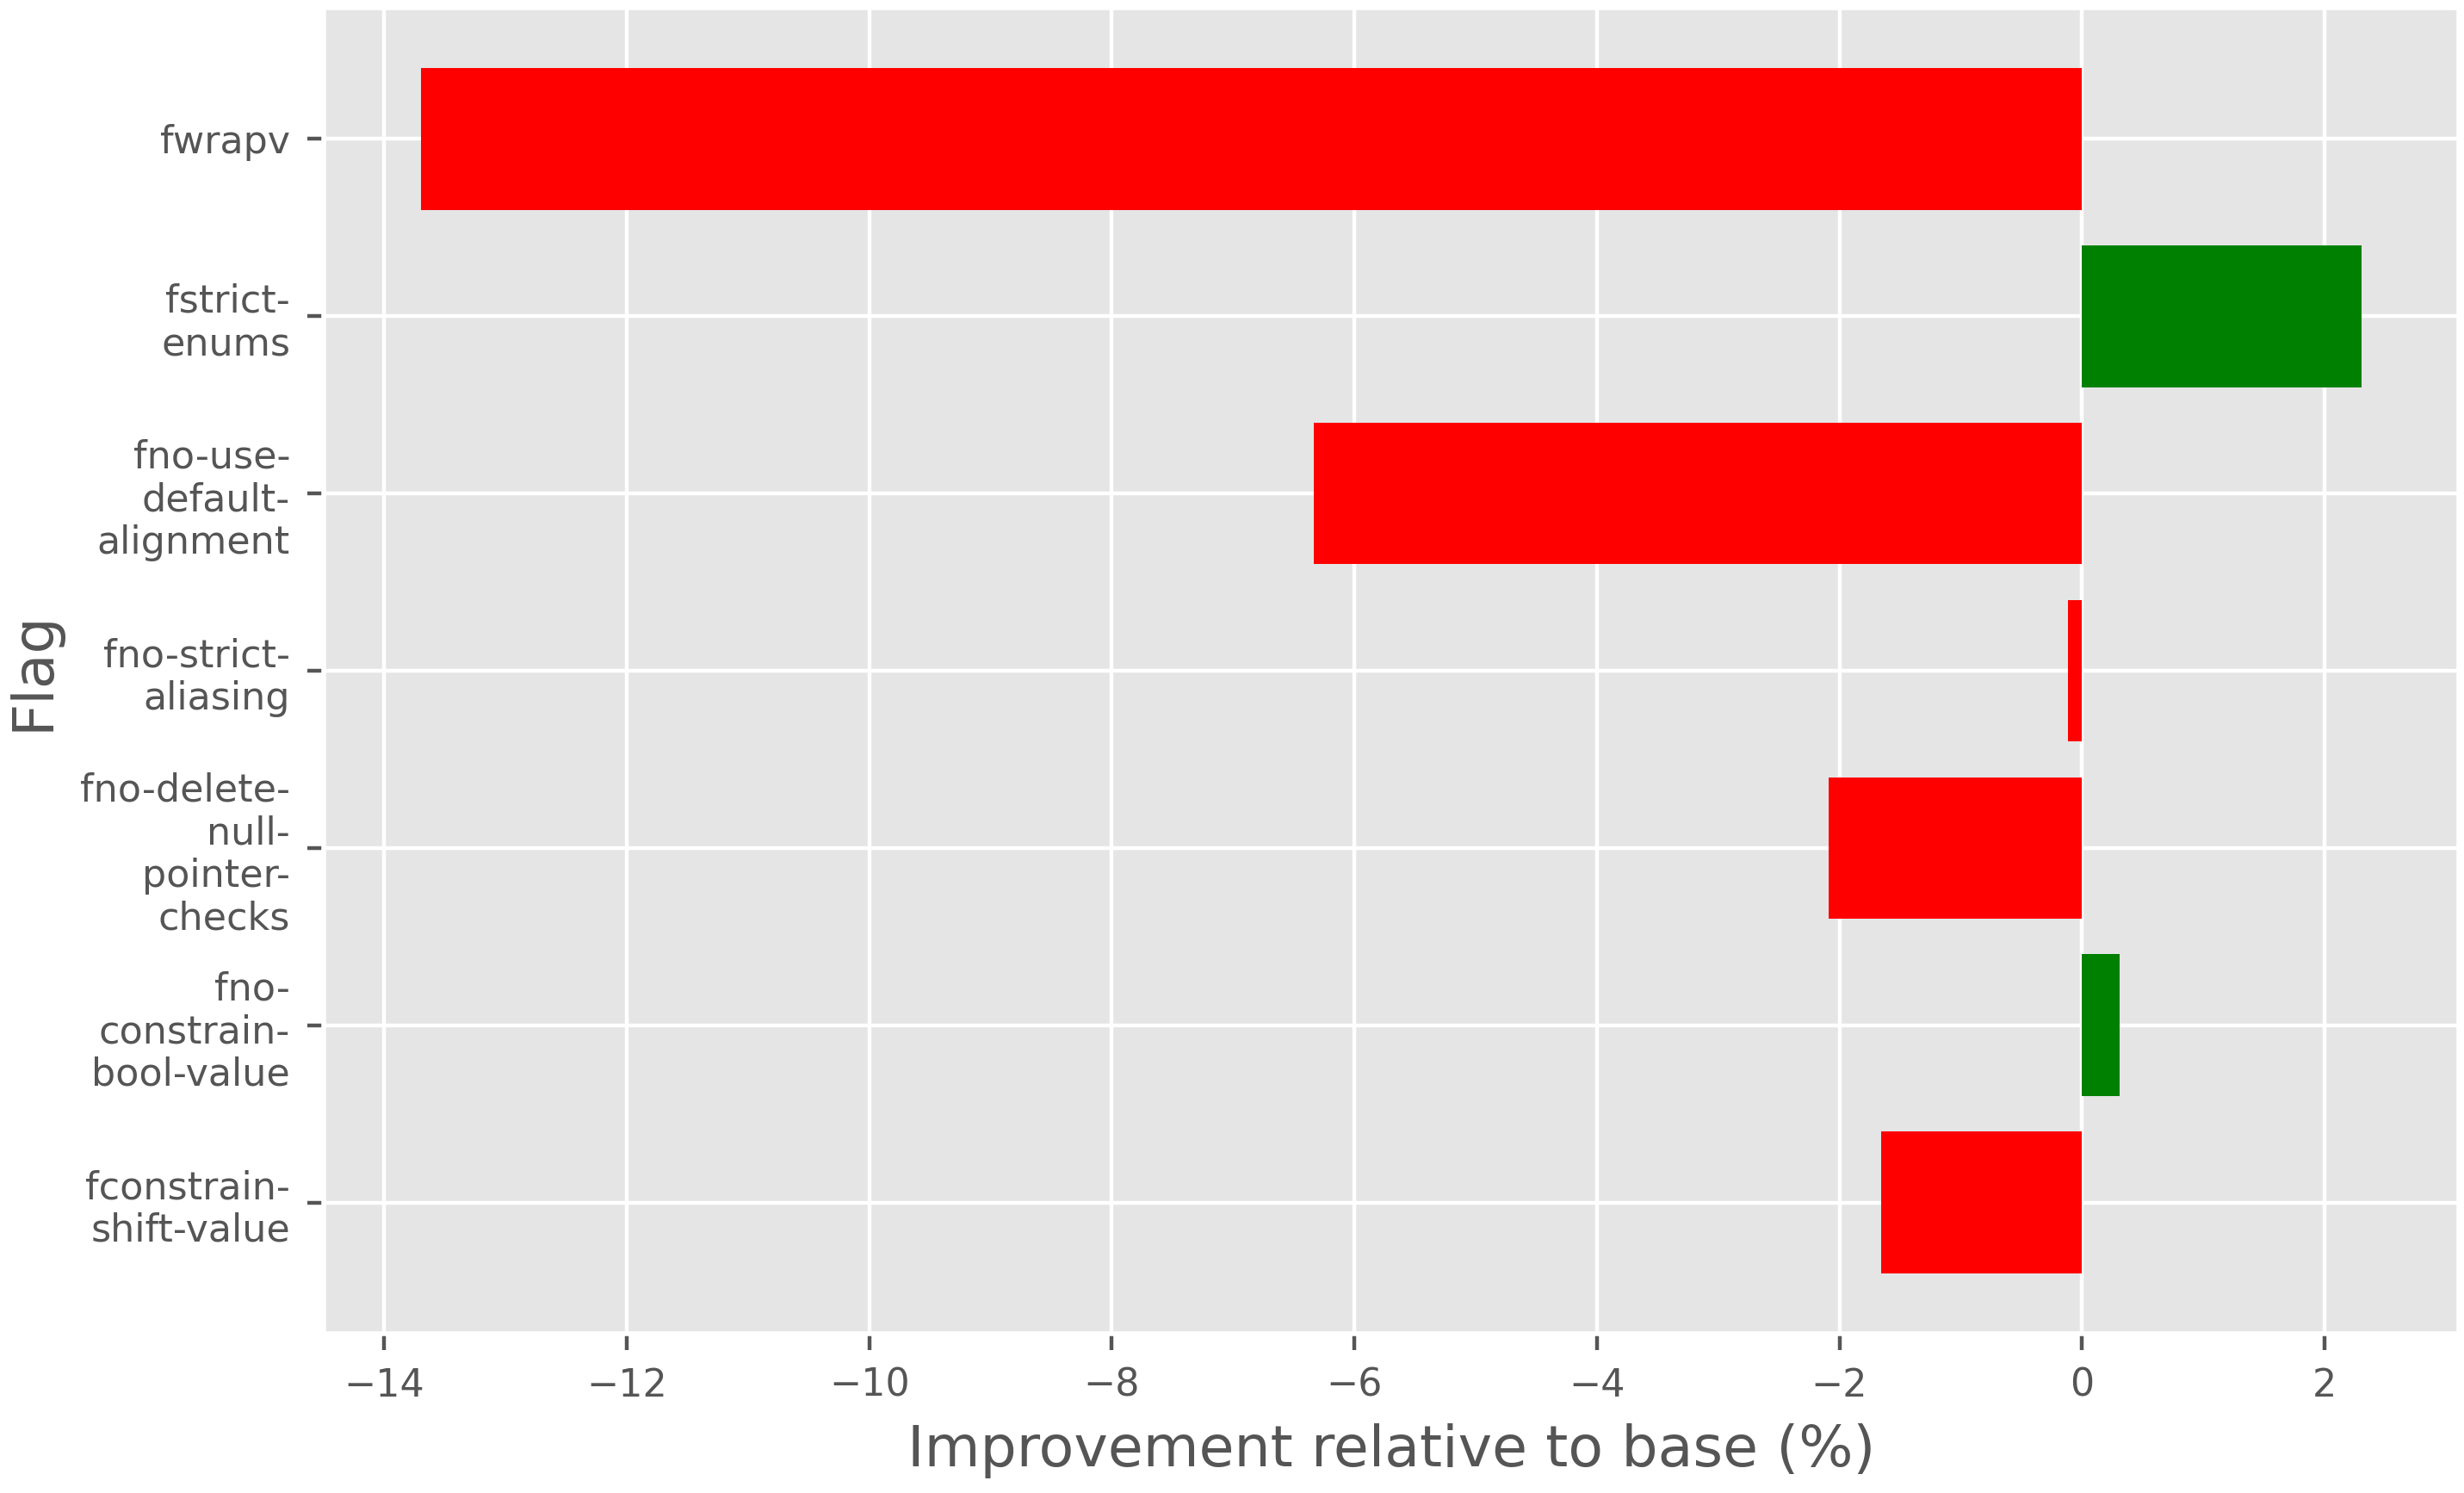
\includegraphics[scale=1.3]{espeak} \\
\caption{eSpeak-NG Speech Engine - Text-To-Speech Synthesis, Baseline: 41.59 Sec} 
\end{figure}

\begin{figure}[h!]
\centering
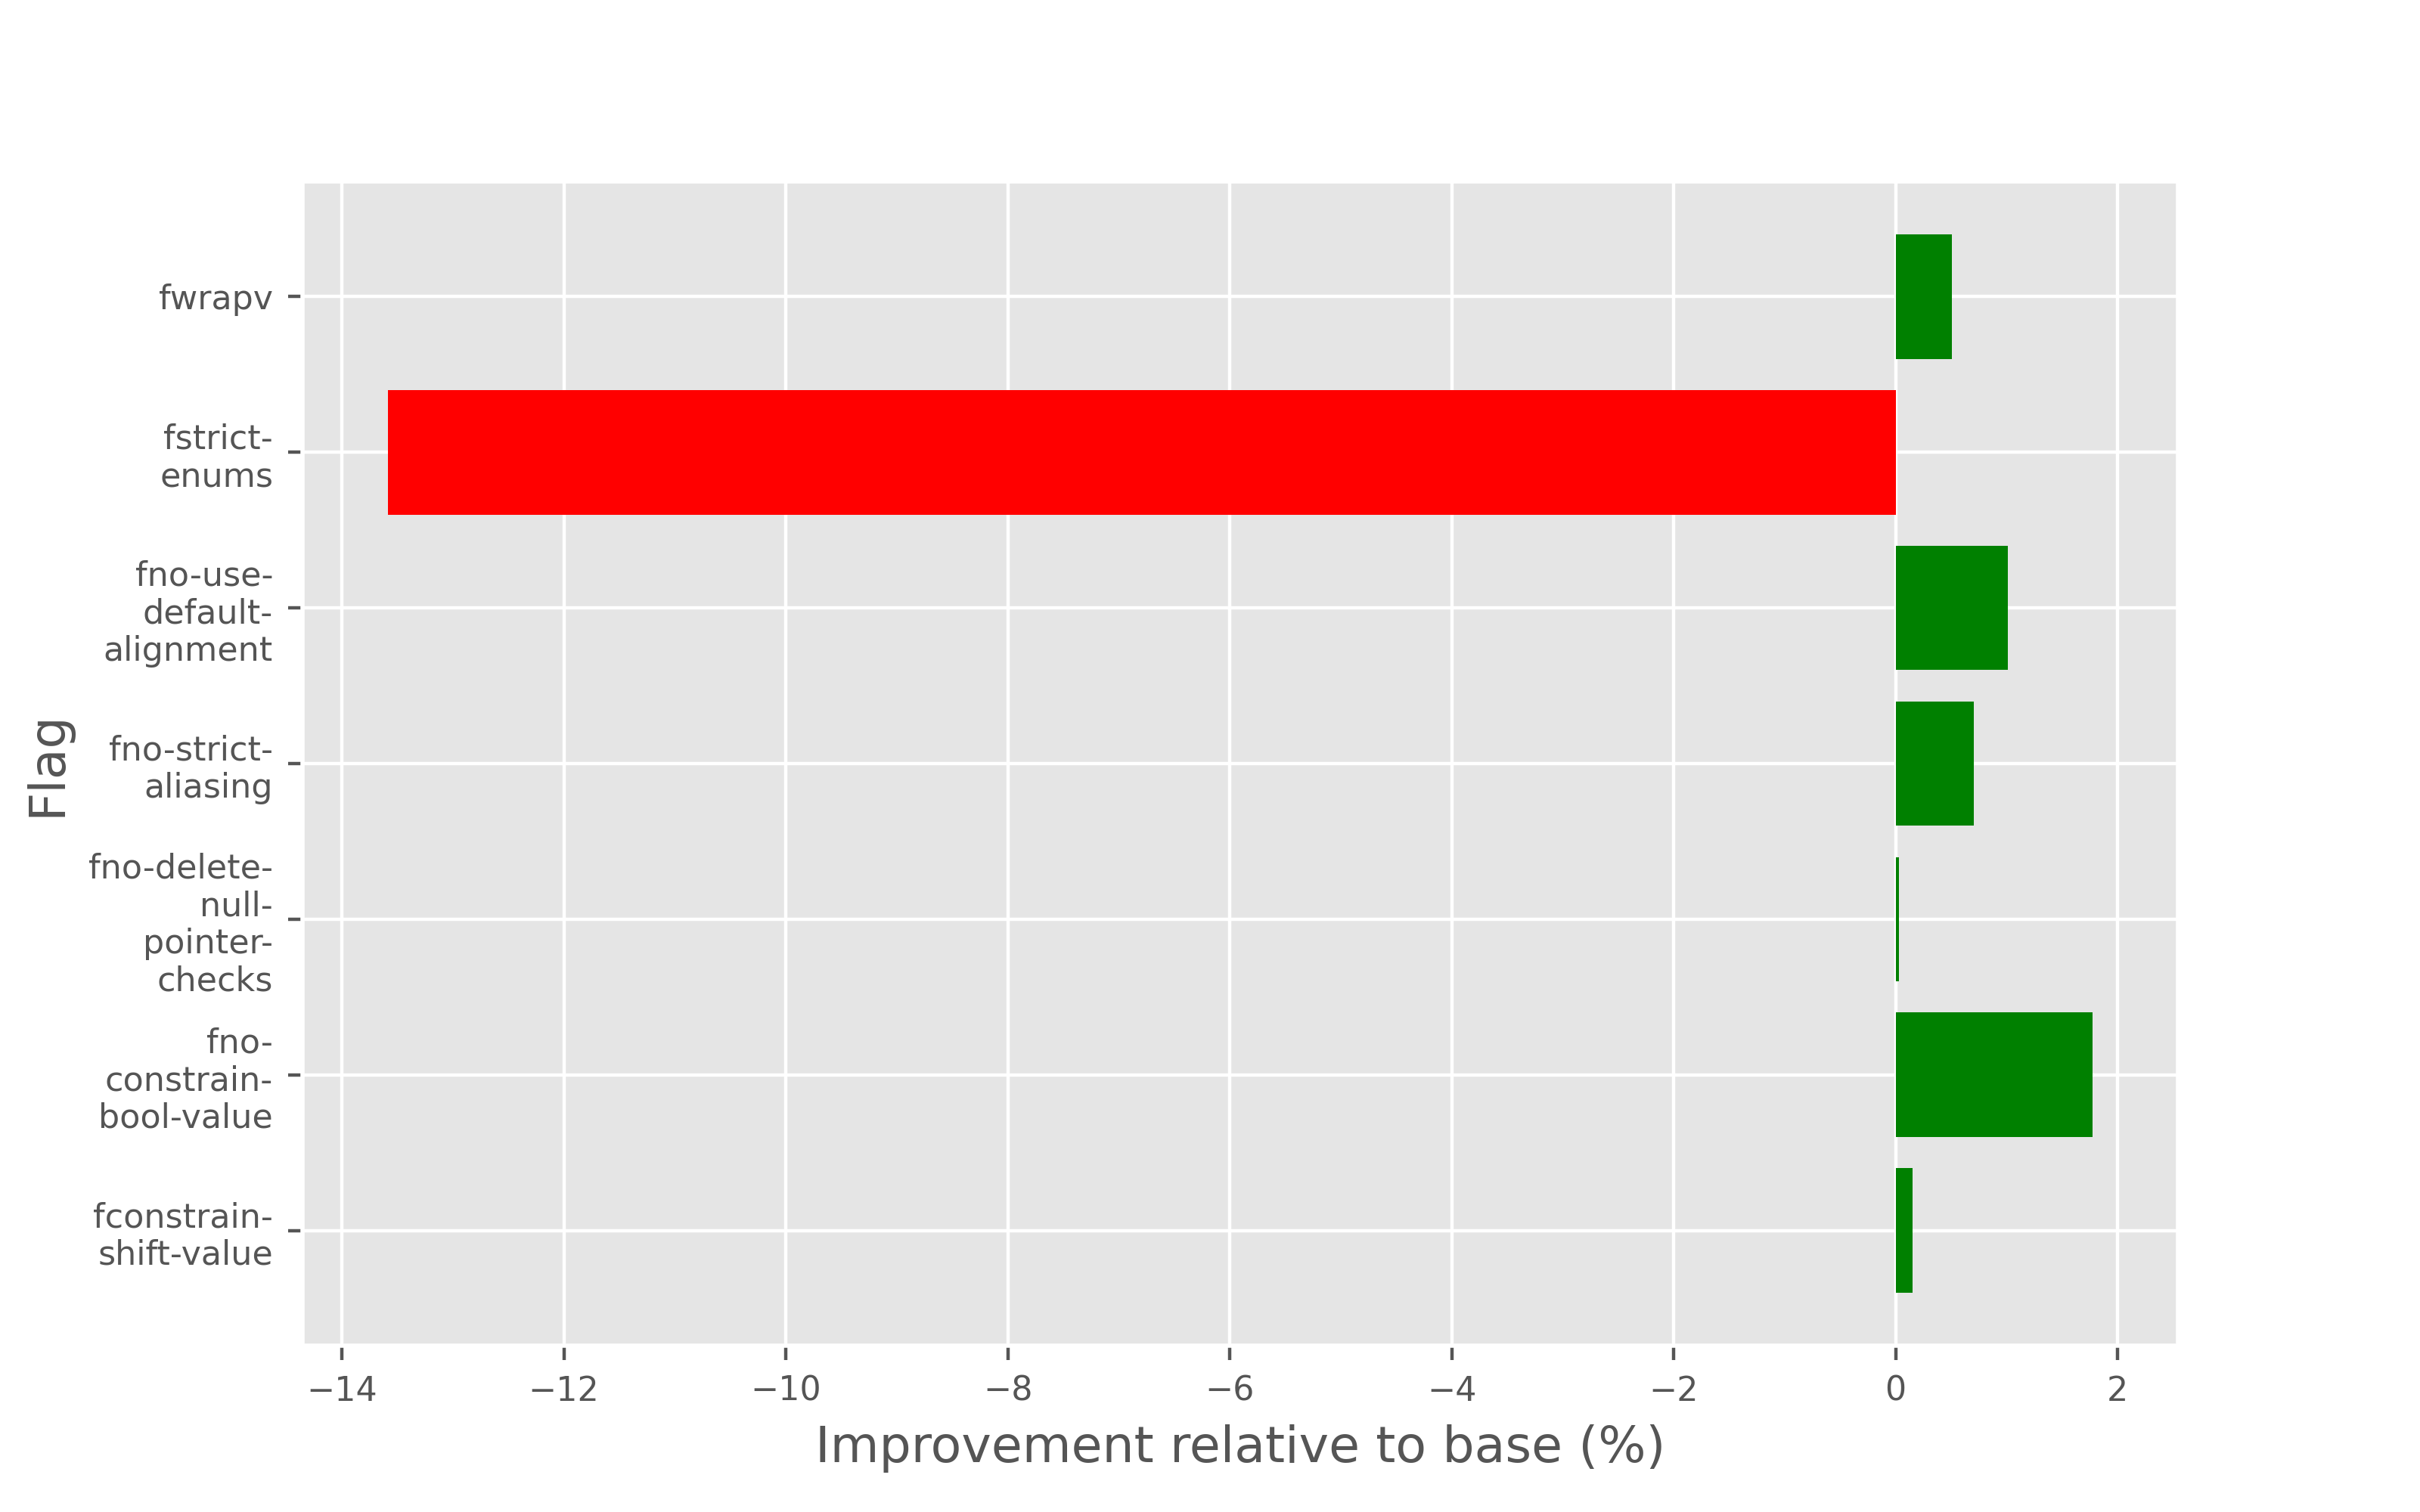
\includegraphics[scale=1.3]{apache} \\
\caption{Apache HTTP Server - Concurrent Requests: 500, Baseline: 102070.20 Reqs/Sec}
\end{figure}

\begin{figure}[h!]
\centering
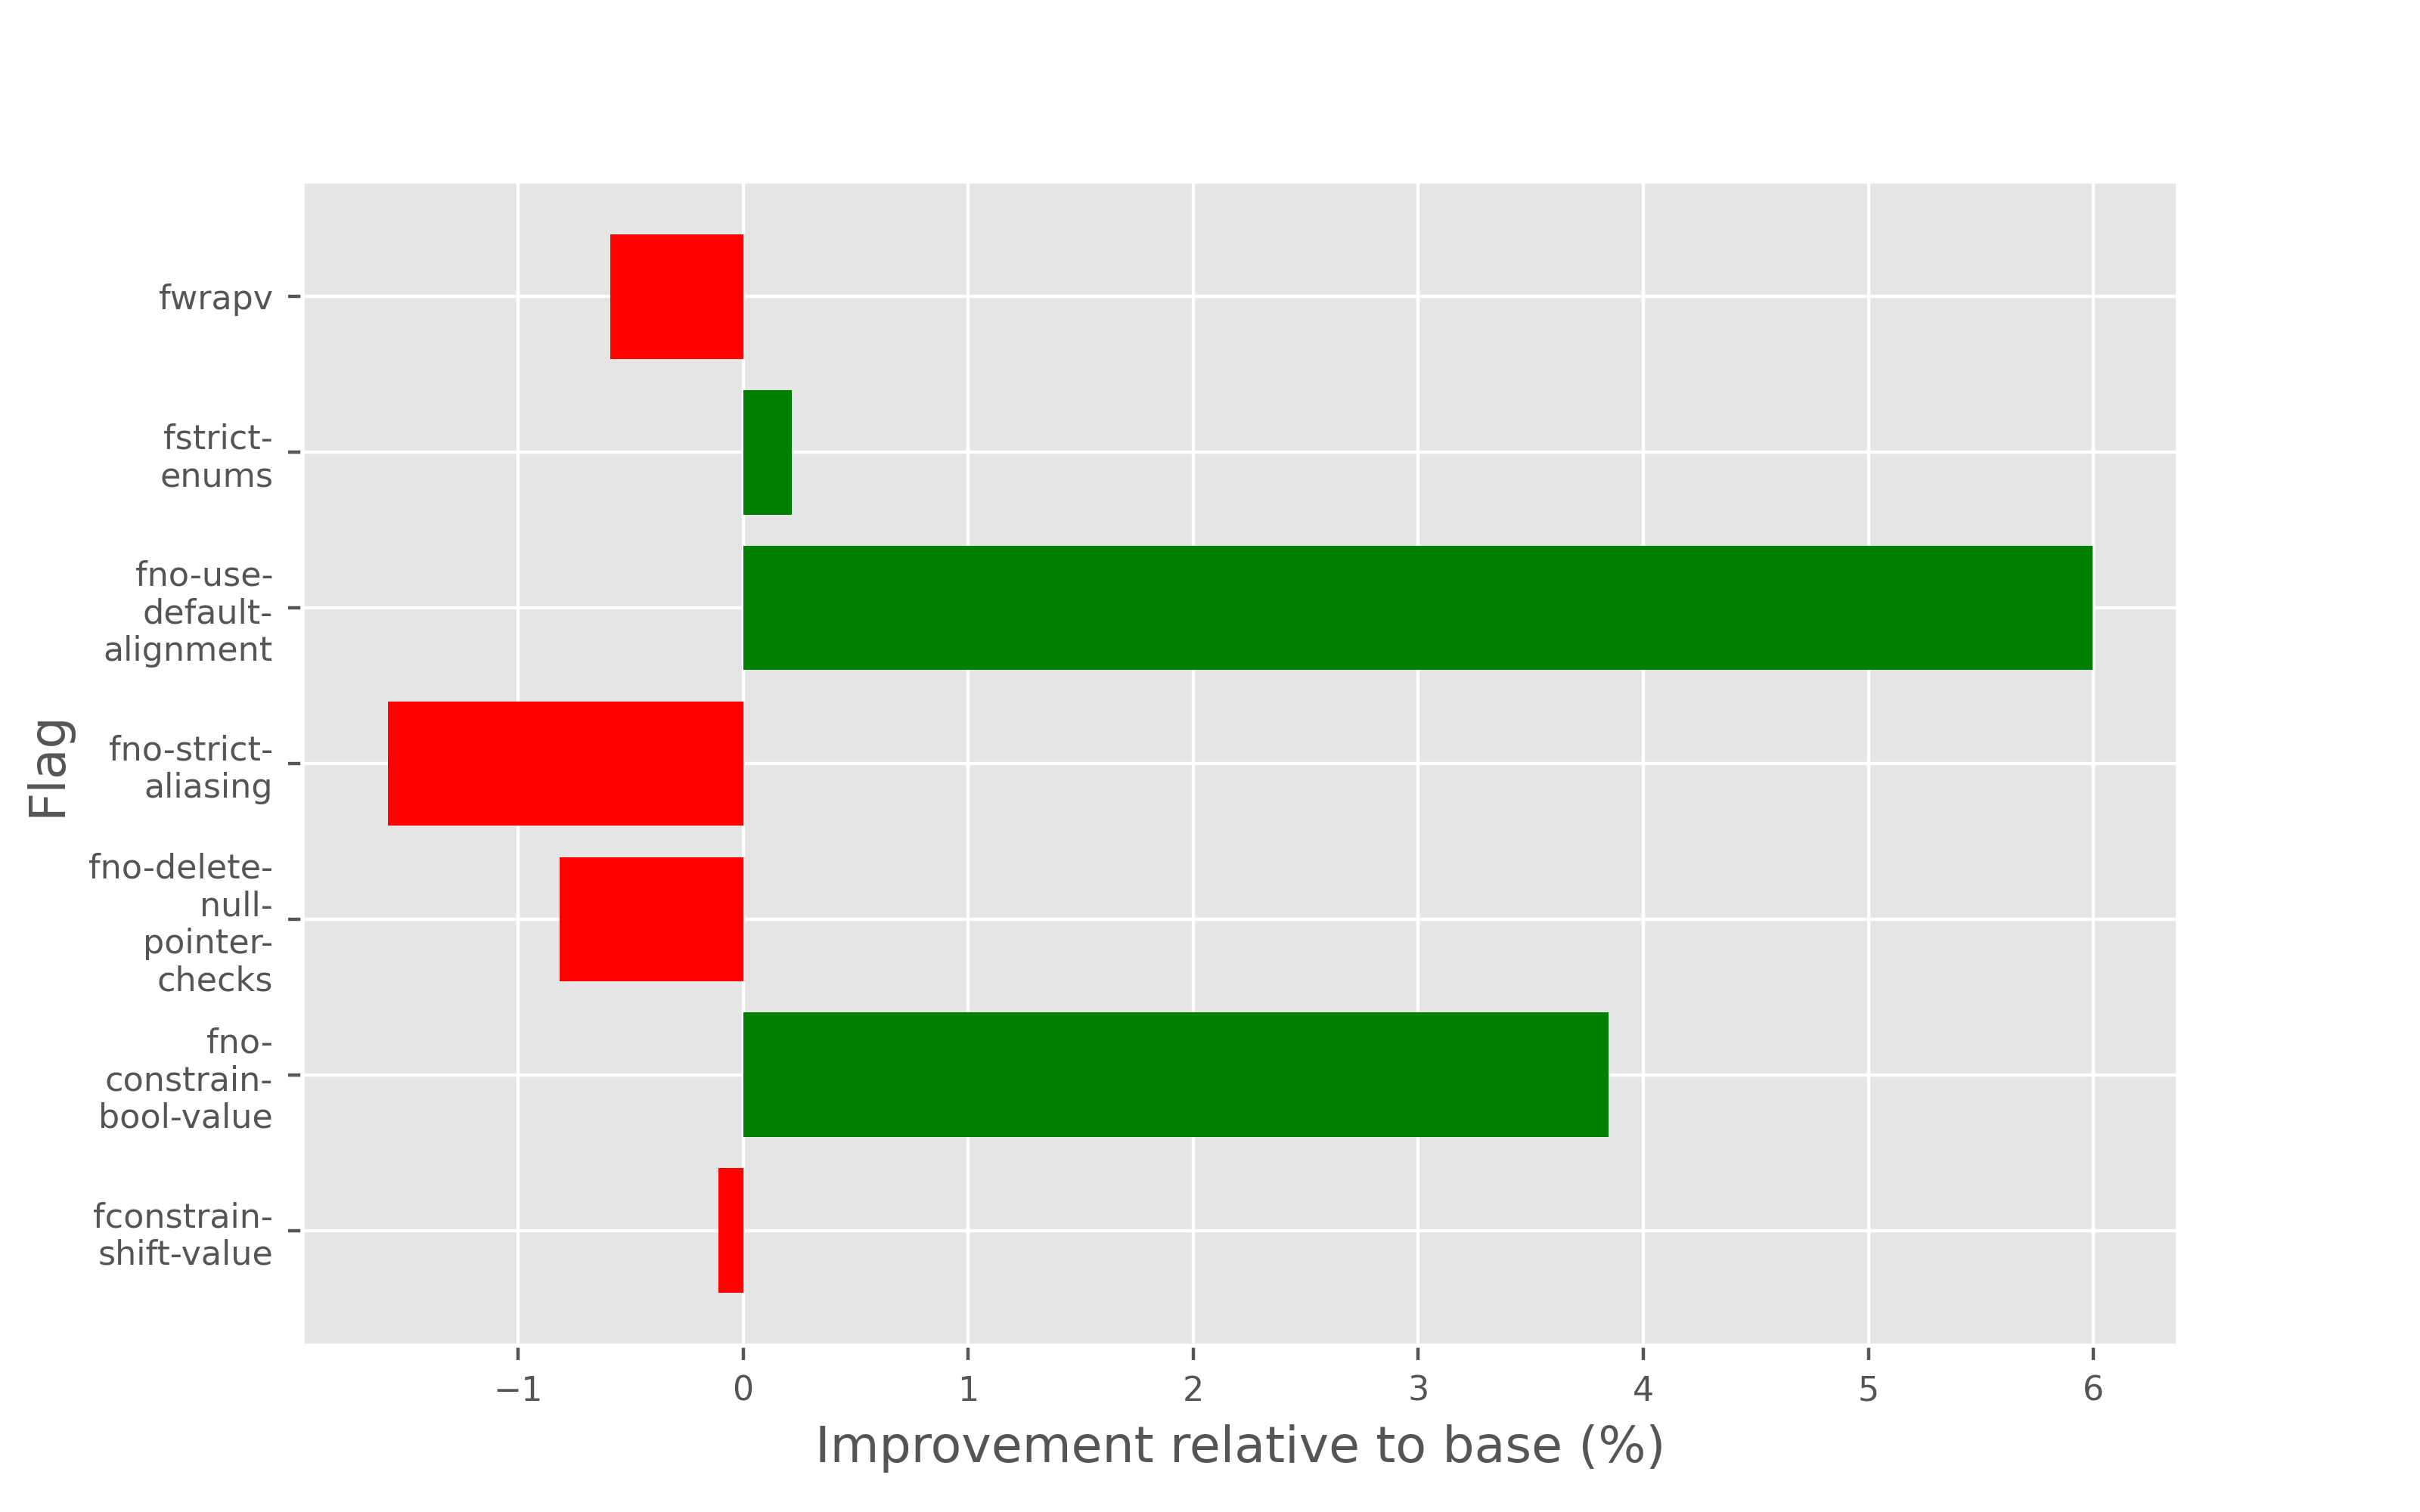
\includegraphics[scale=1.3]{redis} \\
\caption{Redis - Test: SADD - Parallel Connections: 500, Baseline: 1990361.58 Reqs/Sec}
\end{figure}

\begin{figure}[h!]
\centering
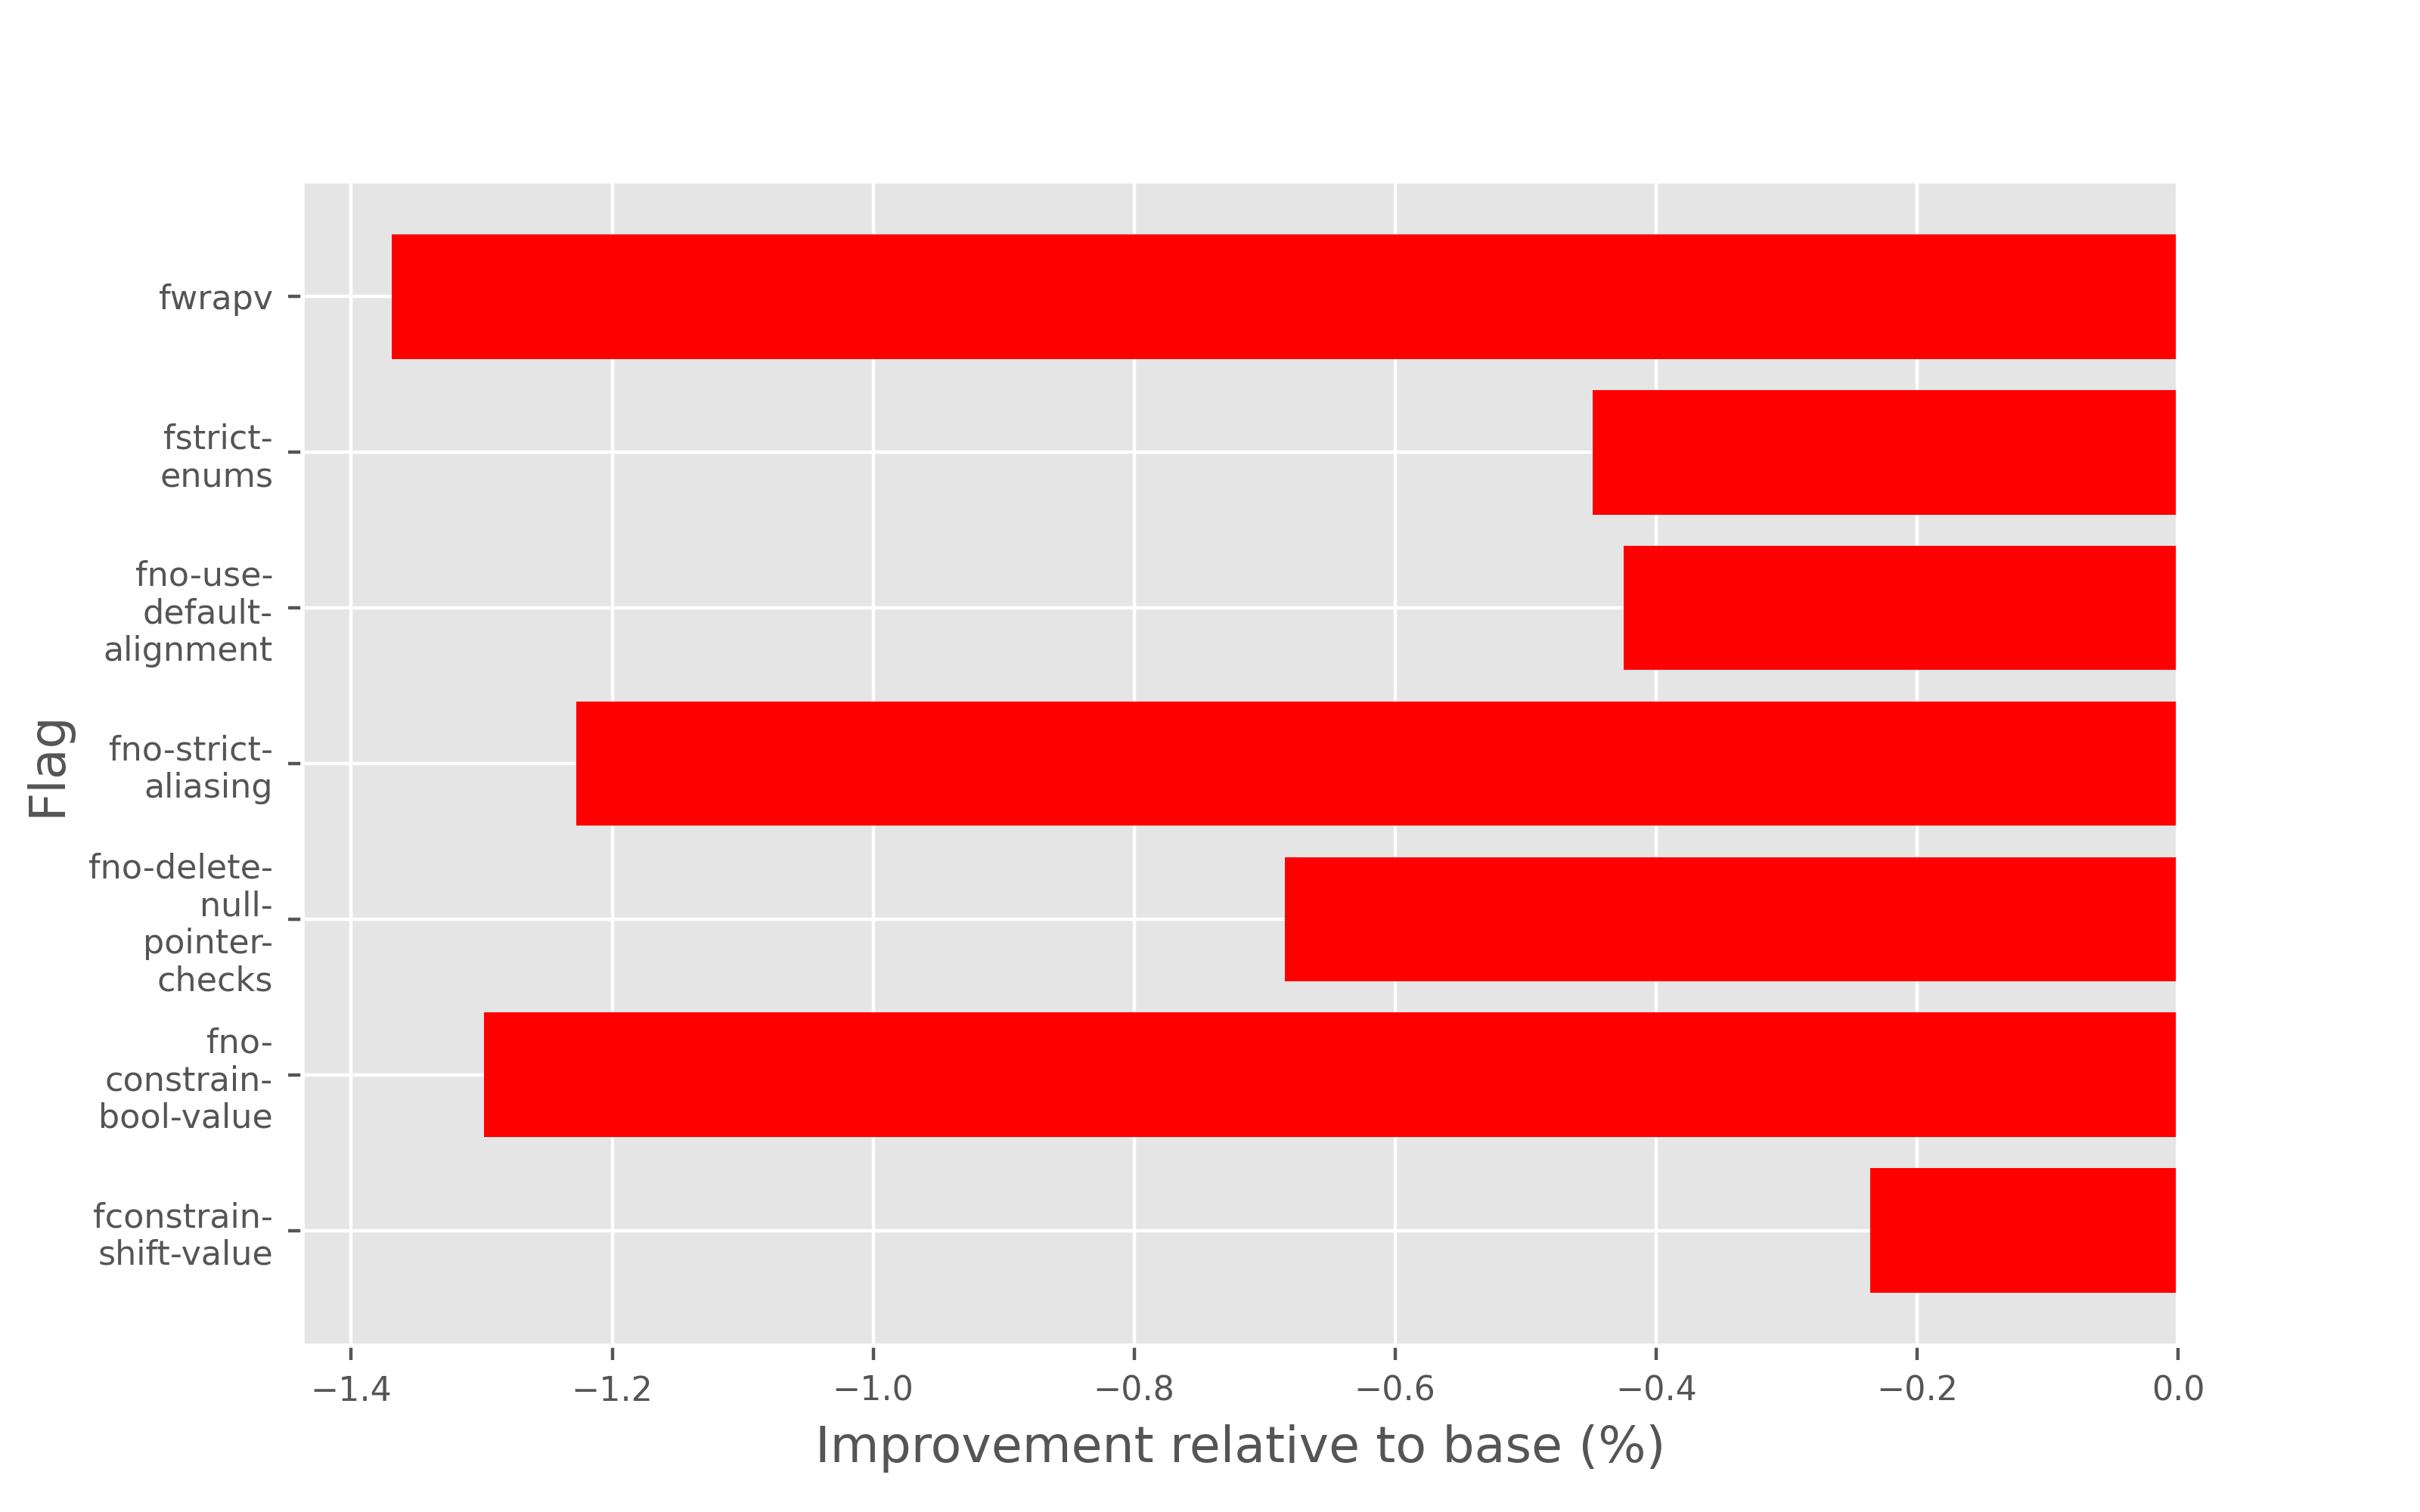
\includegraphics[scale=1.3]{zstd} \\
\caption{CHANGEME}
\end{figure}

\begin{figure}[h!]
\centering
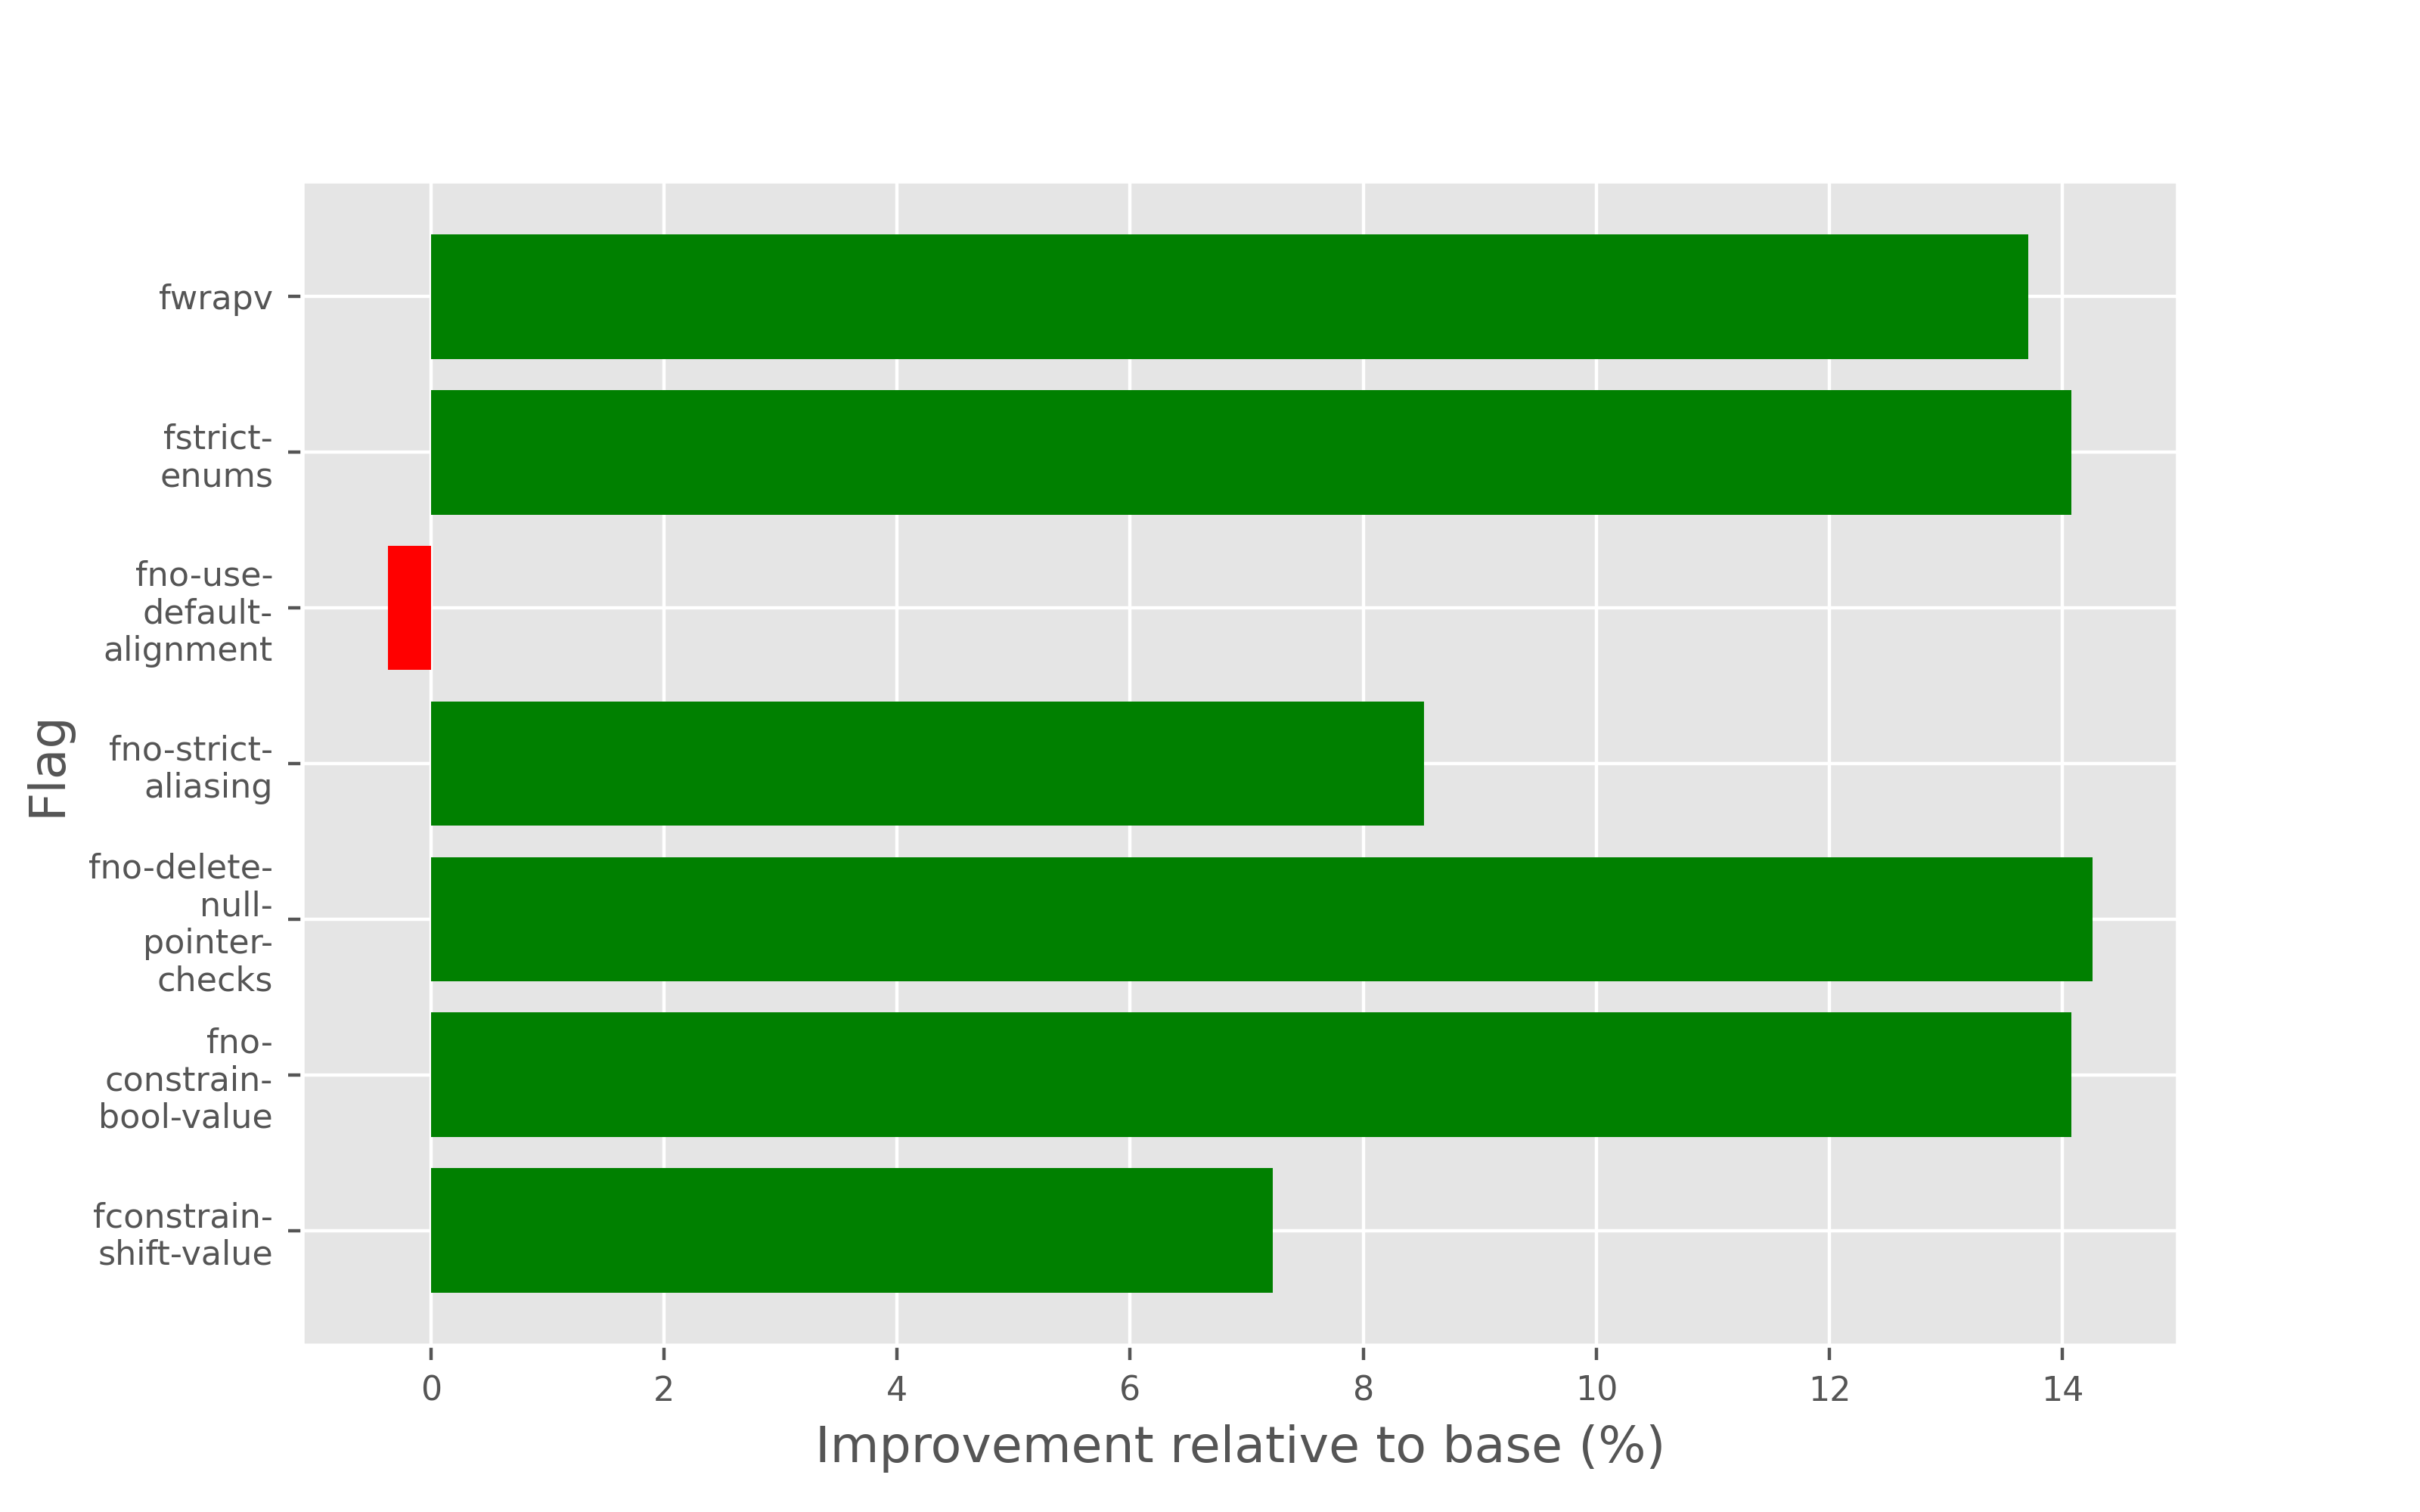
\includegraphics[scale=1.3]{graphicsmagick} \\
\caption{GraphicsMagick - Operation: Rotate, Baseline: 540 Iterations/Min}
\end{figure}

\begin{figure}[h!]
\centering
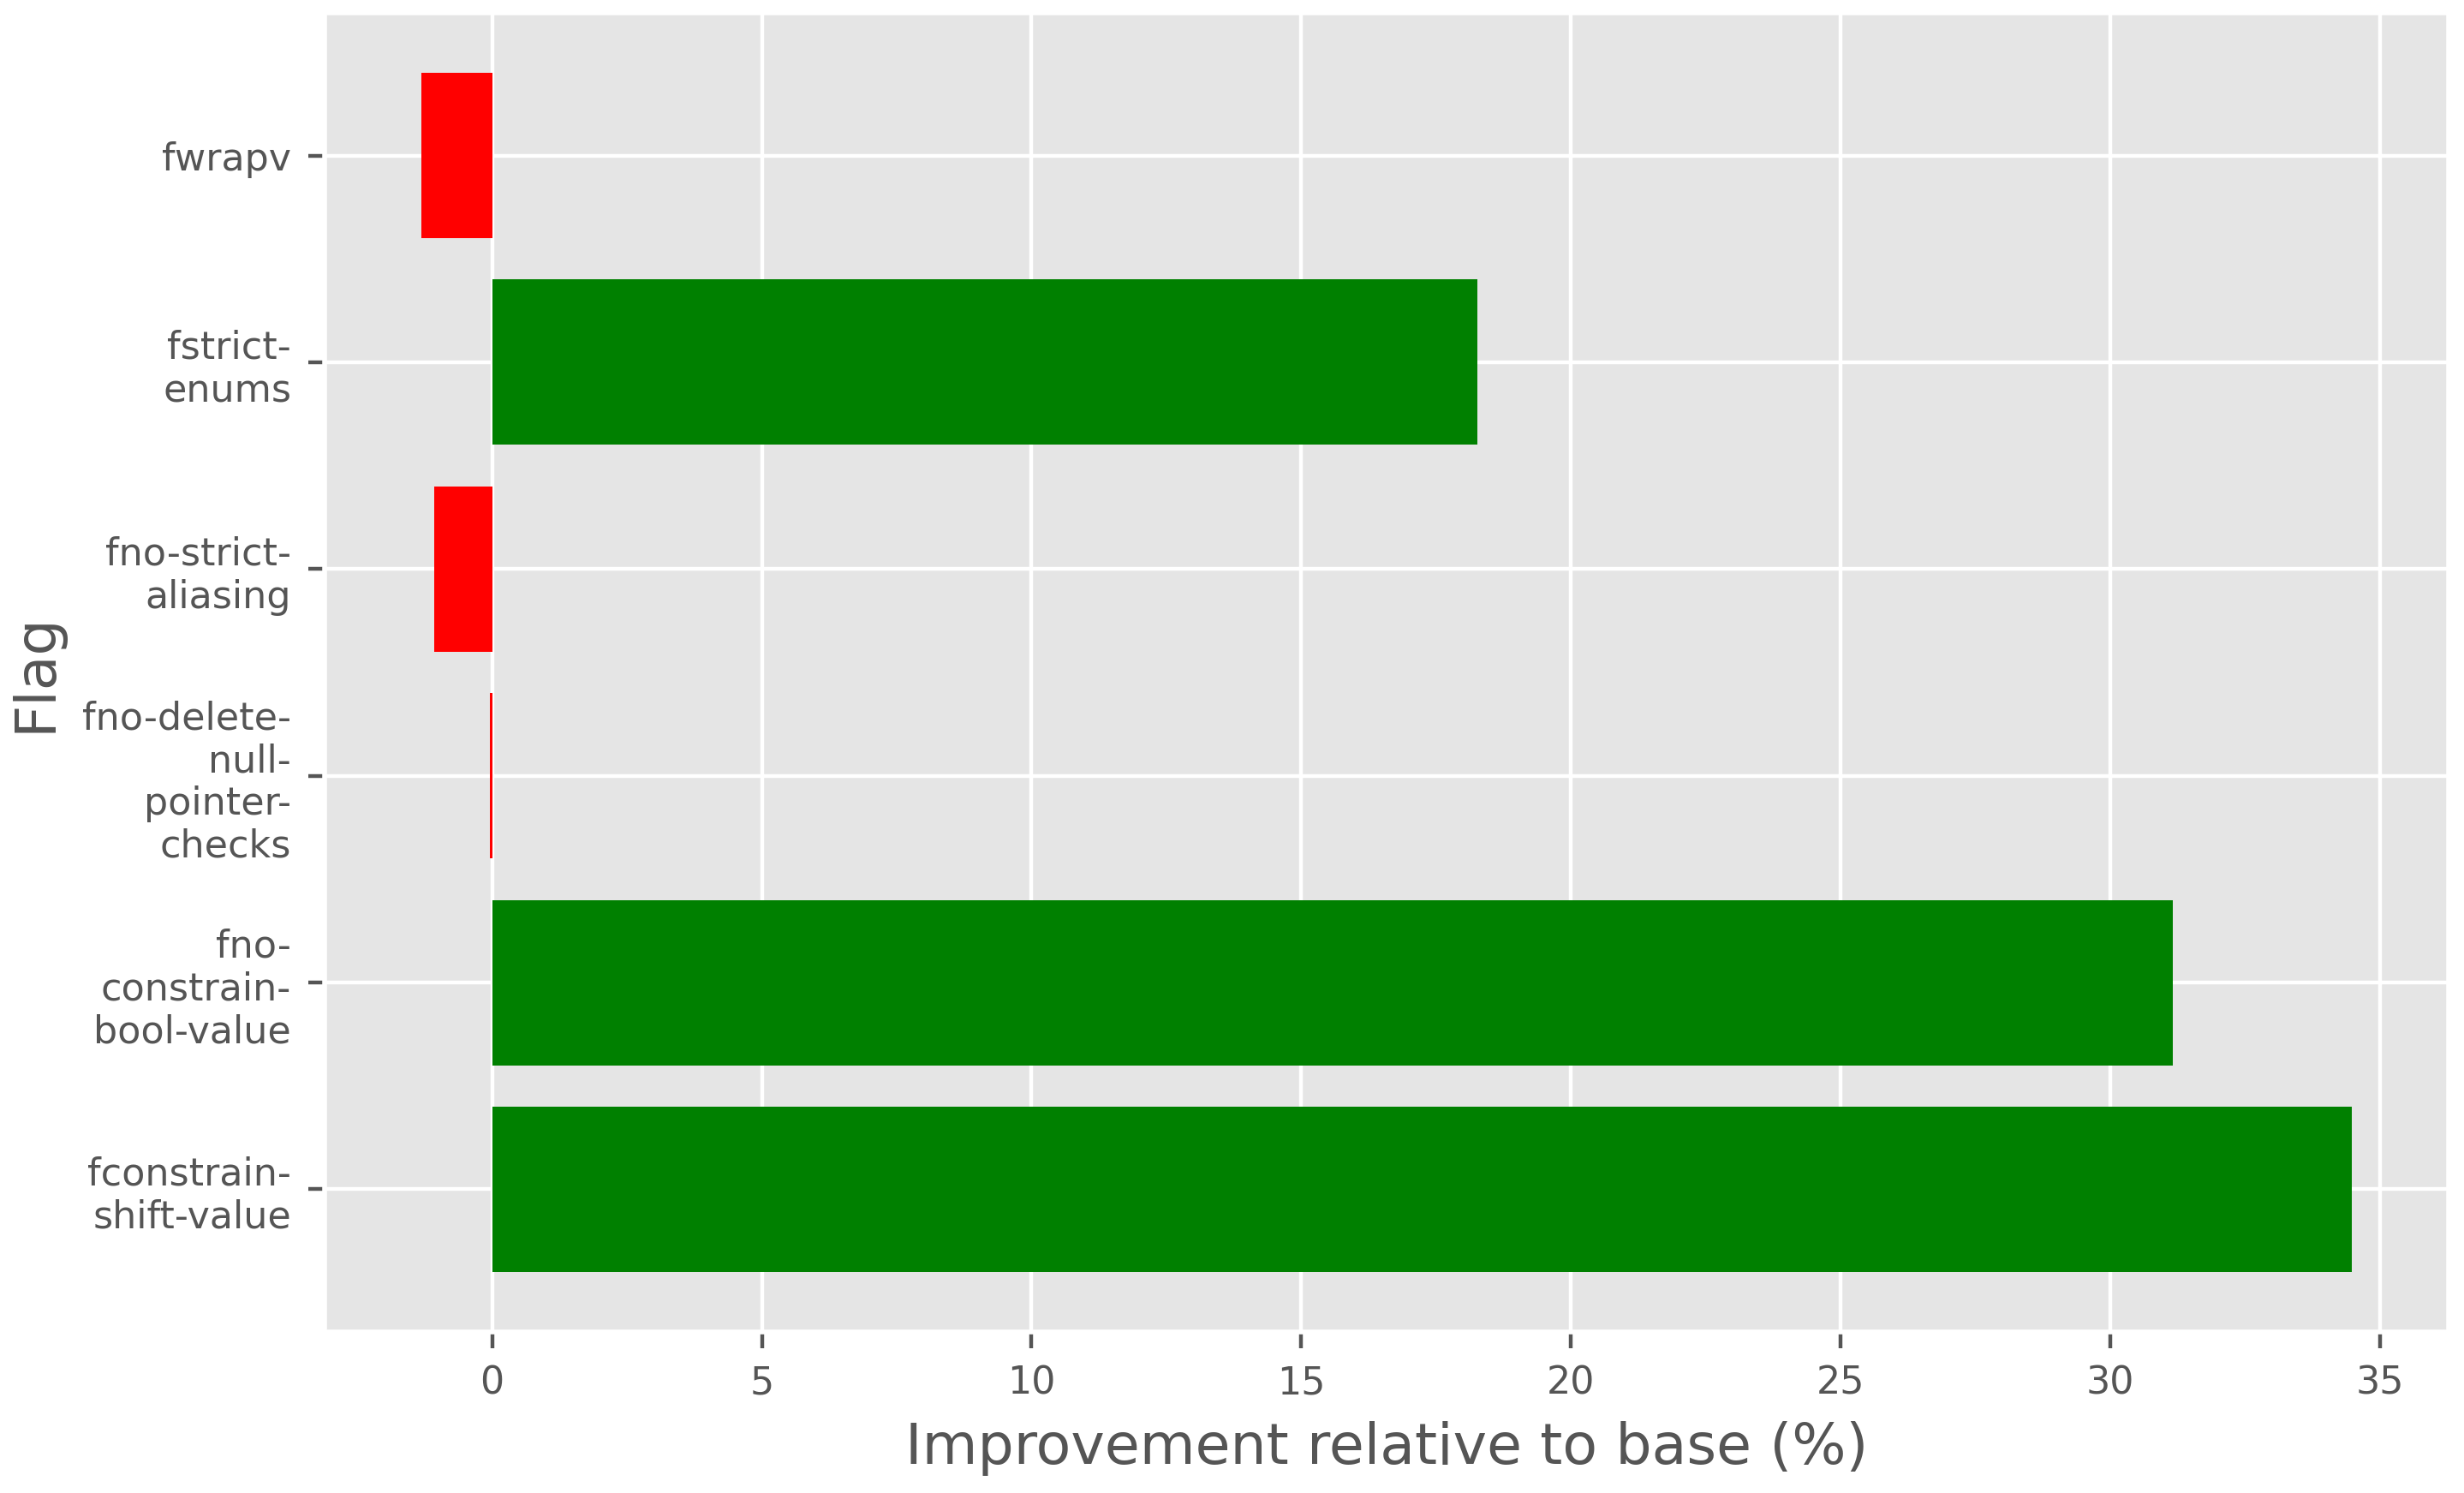
\includegraphics[scale=1.3]{gtkperf} \\
\caption{GtkPerf - GTK Widget: GtkDrawingArea - Pixbufs, Baseline: 170.08 Sec}
\end{figure}

\section{Future work}
\begin{itemize}
\item Clang known UBs are covered, proceed to LLVM UBs
\item Run the benchmarks on different hardware architectures (AMD, ARM)
\item Find a method of discovering new UBs (maybe using Alive)
\item Run the benchmarks taking into account LTO and PGO
\end{itemize}

%%% References

%% Note: use of BibTeX als works!!
\end{multicols}

\end{document}

% TODOS:
% in outliers captions tell the people what is the baseline
% describe the flags
% mention that this is not a sanitizer
% in each caption from sec 3 tell how many values are between 2 and -2
% delete titles from figures
% extract fno-use-default-value correctly because some benchmarks don't have
%  results for this
